\documentclass{article}

\usepackage{verbatim}
\usepackage{amsmath,amsfonts}
\usepackage{enumerate}
\usepackage{fancyvrb}
\usepackage{float}
\usepackage{graphicx}
% \usepackage{fullpage}

\newcommand{\ds}{\ensuremath{\displaystyle}}
\newcommand{\floor}[1]{\ensuremath{\left\lfloor#1\right\rfloor}}
\newcommand{\fracpart}[1]{\ensuremath{\left\{#1\right\}}}

\title{Beginner Test 3}
\author{Stellenbosch Camp 2018}
\date{Time: $4$ hours}


\begin{document}

\maketitle

\begin{enumerate}[1.]

\item 
\textit{Let $AB$ be a chord in a circle with centre $O$, and let $C$ be a point on the larger arc $AB$. Show that $\angle AOB = 2\angle ACB$.}

Proven in lectures; refer to lecture notes.

\vspace{6pt}
\item 
\textit{Factorise the following polynomial completely: \[ (2x+3)^6 -(2x-1)^6. \]}

Using the difference of squares factorisation, we have that
\[
	{(2x + 3)}^6 - {(2x - 1)}^6 = \left( {(2x + 3)}^3 - {(2x - 1)}^3 \right) \left( {(2x + 3)}^3 + {(2x - 1)}^3 \right).
\]
Using the factorisations for differences of cubes, we obtain that
\begin{align*}
	{(2x + 3)}^3 - {(2x - 1)}^3  & = \left( (2x + 3) - (2x - 1) \right) \left( {(2x + 3)}^2 + (2x + 3)(2x - 1) + {(2x - 1)}^2 \right) \\
	 & = 4 \left( (4x^2 + 12x + 9) + (4x^2 + 4x - 3) + (4x^2 - 4x + 1) \right) \\
	 & = 4 ( 12x^2 + 12x + 7 ).
\end{align*}

Similarly using the sum of cubes factorisation, we have that
\[
	{(2x + 3)}^3 + {(2x - 1)}^3 = (4x + 2) (4x^2 + 4x + 13).
\]

The factorisation is thus $8(2x + 1)(4x^2 + 4x + 13)(12x^2 + 12x + 7)$.

\item 
\textit{How many different rearrangments are there of the word TARTAGLIA?}

There are
\[
	\frac{9!}{2! \times 3!}
\]
arrangements.

\vspace{6pt}
\item 
\textit{In the figure $ABC$ is a tangent to the circumscribed circle of $\triangle PBG$. $PS$ and $DG$ are both parallel to $ABC$. Chords $BP$ and $BS$ cut $DG$ at $E$ and $F$ respectively. Prove that:
\begin{enumerate}[a.]
  \item $\angle G_1 = \angle P_1$
  \item $\triangle BGP$ is similar to $\triangle BEG$
  \item $BG^2 = BP \times BE$
  \item $\frac{BG^2}{BP^2} = \frac{BF}{BS}$
\end{enumerate}}

\begin{figure}[H]
  \centering
  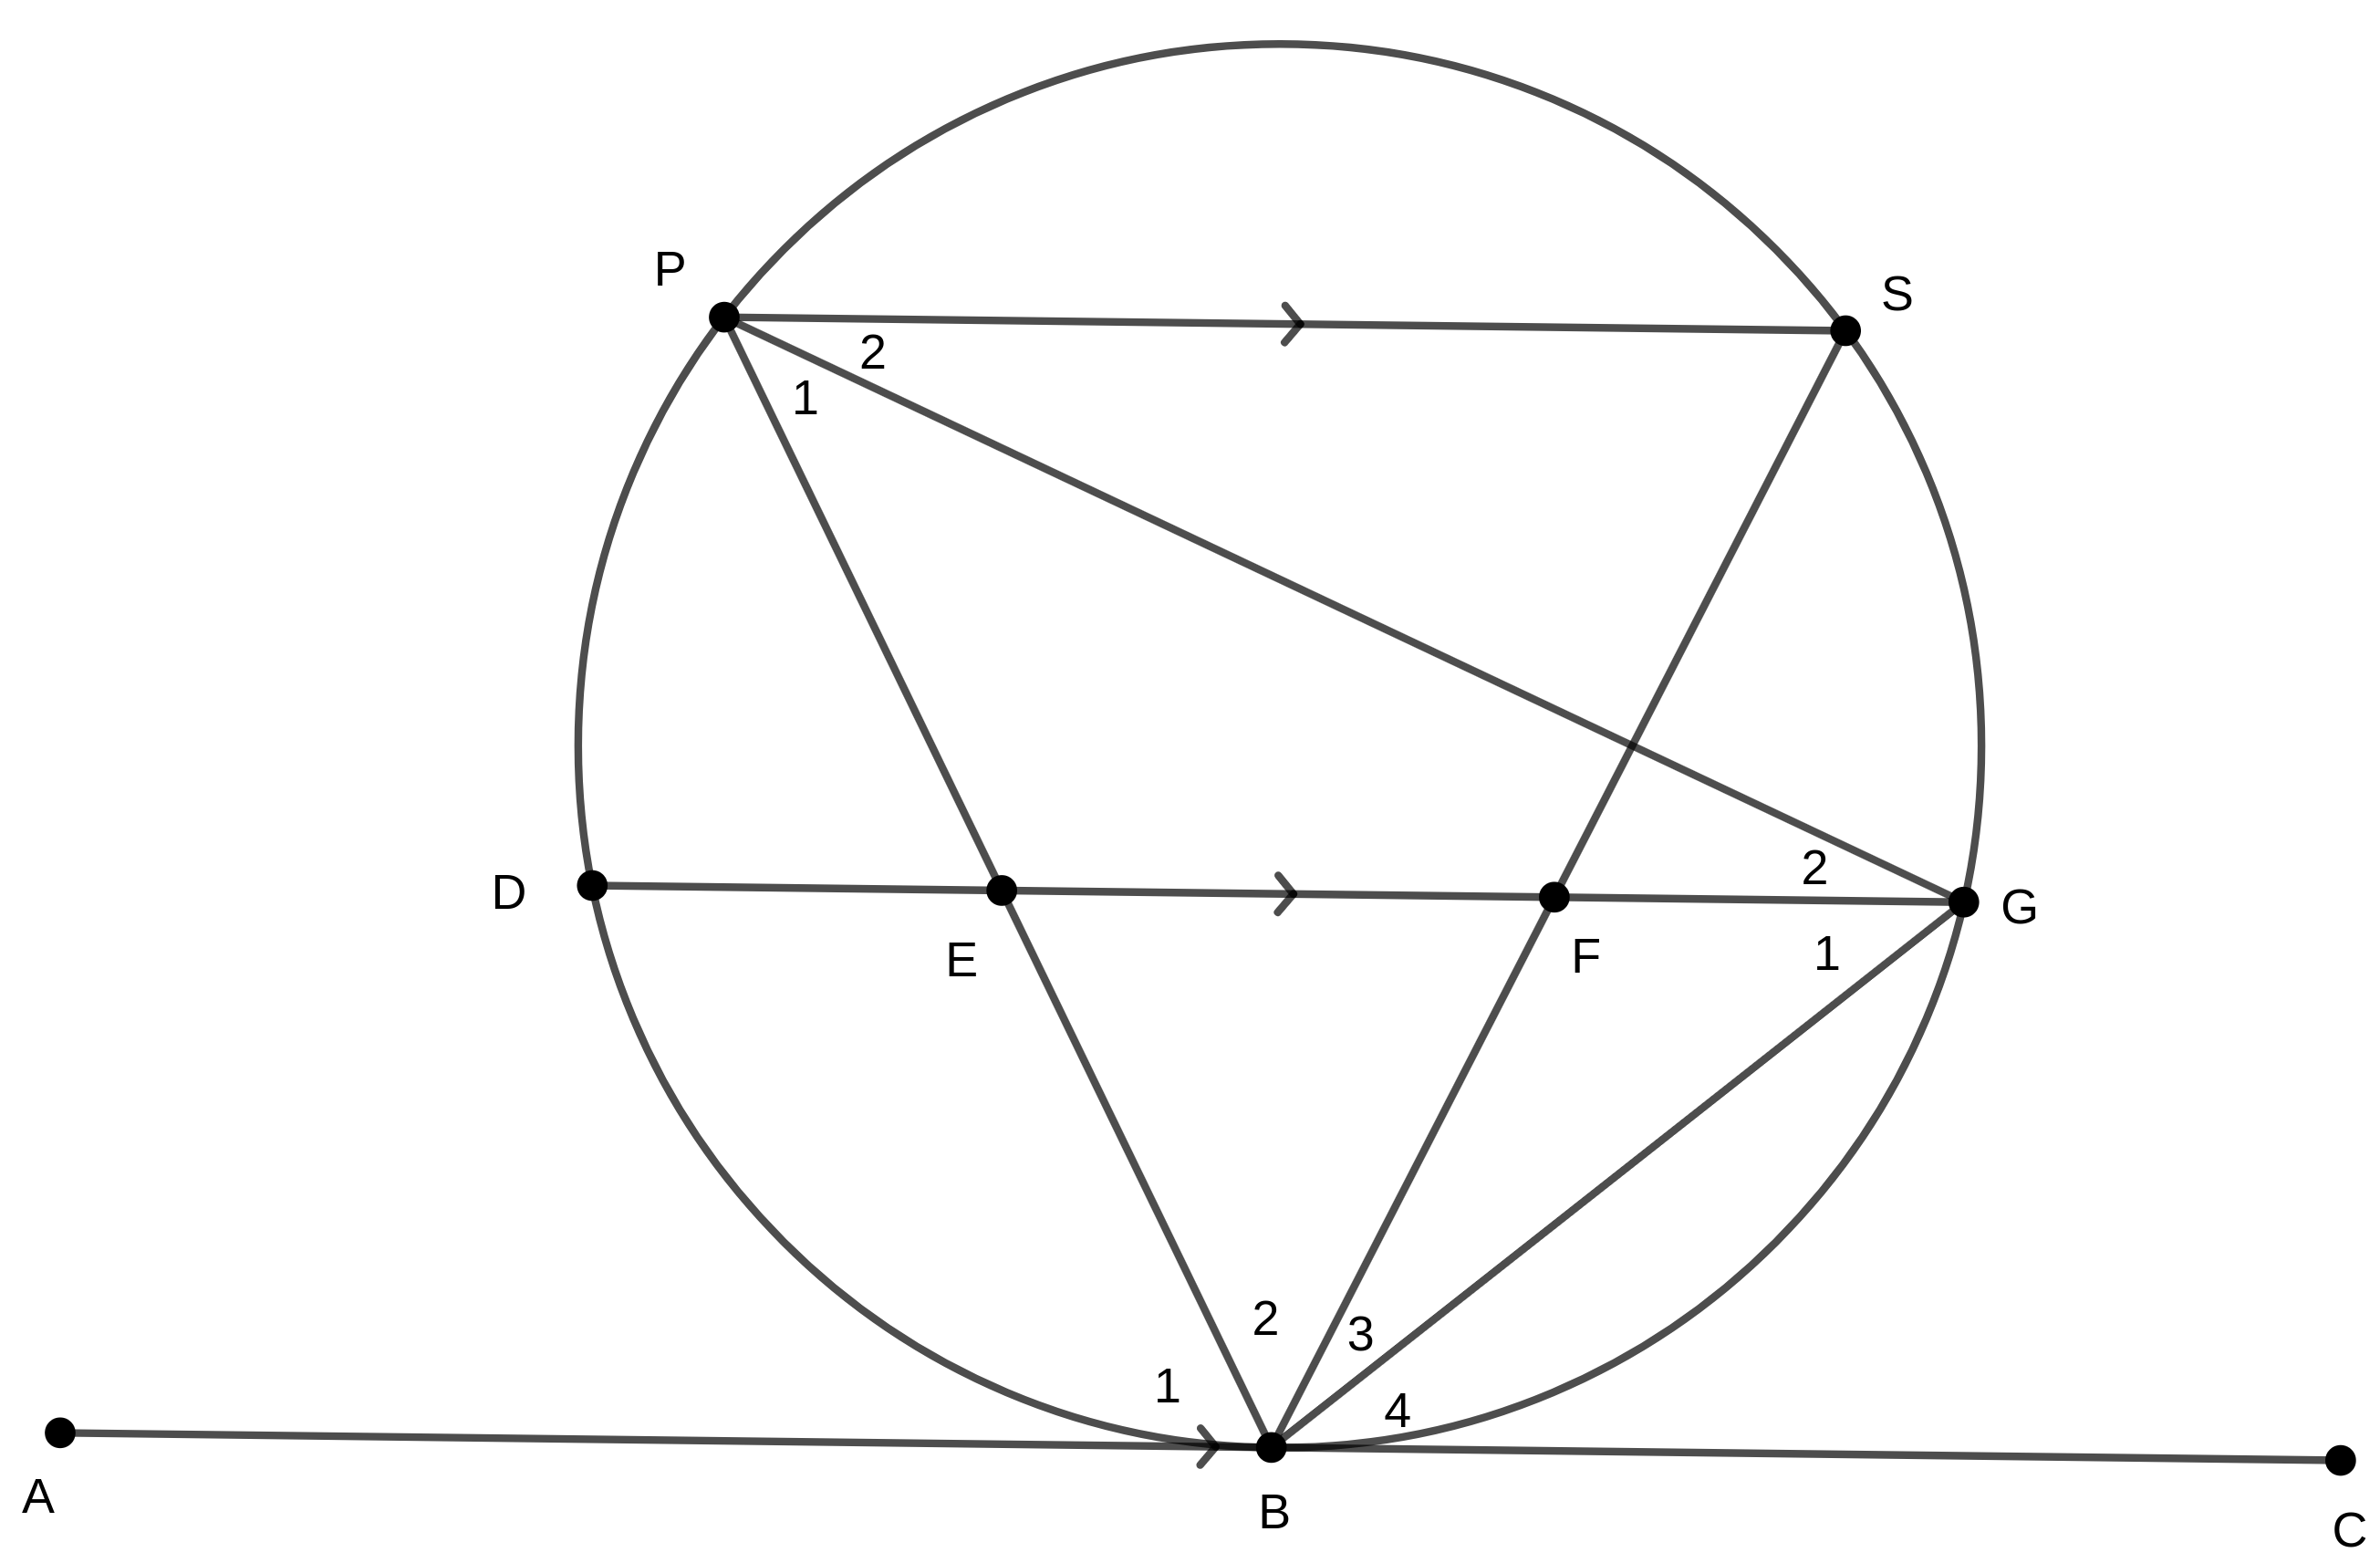
\includegraphics[width = 0.8\linewidth]{test3_geometry1.png}
\end{figure}
 
\begin{enumerate}[a.]
  \item We have that $G_1 = B_4$ (alternating angles) $= P_1$ (tan-chord).
  \item Since $G_1 = P_1$ and $\angle GBP$ is common to both triangles, the two triangles have two pairs of angles equal and hence are similar.
  \item Since $\triangle BGP$ is similar to $\triangle BEG$, we have that
  \[
		\frac{BG}{BE} = \frac{BP}{BG}
  \]
  which is equivalent to the desired result.
  \item We know that
  \[
		\frac{{BG}^2}{{BP}^2} = \frac{BP \times BE}{{BP}^2} = \frac{BE}{BP} = \frac{BF}{FS}
  \]
  where the last equality follows because $\triangle BFE$ is similar to $\triangle BSP$.
\end{enumerate}

\vspace{6pt}
\item 
\textit{Consider a game wherein two players Emma and Dylan take turns to take between 1 and 7 stones, inclusive, from a pile which starts with 2018 stones. If Emma plays first, does one of the players have a winning strategy, and if so what is it?}

Emma has a winning strategy. On her first turn, she takes $2$ stones. Thereafter, if Dylan takes $n$ stones on his turn then Emma responds by taking $8 - n$ stones on her turn. The number of stones is then always a multiple of $8$ after Emma's turn and is never a multiple of $8$ after Dylan's turn. In particular, the number of stones can never be $0$ after Dylan's turn. Since the game must eventually end, can not end in a draw, and can not be won by Dylan, it must be Emma who wins.

\vspace{6pt}
\item 
\textit{Determine all solutions $(x,y)$ of the system of equations
\begin{align*}
  \frac{4}{x} +\frac{5}{y^2} &= 12, \\
  \frac{3}{x} +\frac{7}{y^2} &= 22.
\end{align*}}

Subtracting $3$ times the first equation from $4$ times the second gives us that
\[
	\frac{13}{y^2} = 52
\]
and so $y^2 = 1/4$. Substituting this back into the equation gives us that $4/x = 12 - 20 = -8$ and so $x = -1/2$. The solutions are thus $(x, y) = (-1/2, -1/2)$ and $(x, y) = (-1/2, 1/2)$.

\item 
\textit{Suppose $k$ is a positive integer that does not divide $2008$. Let $[x]$ denote the greatest integer less than or equal to $x$. For example, $[11.75] = 11$ and $[\pi] = 3$. What is the maximum possible value of $k \times \left[\frac{2018}{k}\right]$?}

Let $2018 = kq + r$ where $0 \leq r < k$. Since $k$ does not divide $2018$, we have that $0 < r$. Then we have that
\[
	\left[ \frac{2018}{k} \right] = \left[ \frac{kq + r}{k} \right] = \left[ q + \frac{r}{k} \right] = q.
\]
We thus want to find the largest possible value of $kq = 2018 - r$. This corresponds to the smallest possible value of $r$, which is equal to $1$, and so the maximum possible value of
\[
	k \left[ \frac{2018}{k} \right]
\]
is $2017$. Equality occurs for any $k$ such that $2018$ leaves a remainder of $1$ when divided by $k$, for example $k = 2017$.


\vspace{6pt}
\item % 
\textit{The student lockers at Olympic High are numbered consecutively beginning with locker number 1. The plastic digits used to number the lockers cost $3$ cents per piece. Thus, it costs $3$ cents to number locker $9$ and $6$ cents to number locker $42$. If it costs R206.91 to label all the lockers, how many lockers are there at the school?}

We claim there are 2001 lockers. Indeed, the total cost comes to:

\begin{equation*}
    3c \cdot (9 - 0) + 6c \cdot (99 - 9) + 9c \cdot (999 - 99) + 12c \cdot (2001 - 999) = 20691c
\end{equation*}

\vspace{5mm}

\vspace{6pt}
\item 
\textit{Consider the function $f(x) = \frac{1}{1-x}$ and its iterates $f^r$ defined as
\begin{align*}
  f^1(x) &= f(x) \\
  f^2(x) &= f(f(x)) \\
  f^3(x) &= f(f(f(x))) \\
  f^4(x) &= f(f(f(f(x)))),
\end{align*}
and so on. Calculate the value of $f^{2018}(2018)$.}

Note that
\[
	f^1(x) = \frac{1}{1 - x},
\]
\[
	f^2(x) = \frac{1}{1 - \frac{1}{1 - x}} = \frac{x - 1}{x}
\]
and
\[
	f^3(x) = f^2(f(x)) = \frac{\frac{1}{1 - x} - 1}{\frac{1}{1 - x}} = x
\]

We thus have that 
\[
	f^{2018} = f^3(f^{2015}(x)) = f^{2015}(x) = f^3(f^{2012}(x)) = f^{2012}(x) = \cdots = f^2(x) = \frac{x-1}{x}
\]
and so
\[
	f^{2018}(2018) = \frac{2018 - 1}{2018} = \frac{2017}{2018}.
\]

\vspace{6pt}
\item % UK IMO 2001 IMO training problem sheet
\textit{Given the equation $x^{2018} = y^x$,
\begin{enumerate}
  \item find all pairs $(x,y)$ of solutions with $x$ prime and $y$ a positive integer;
  \item find all pairs $(x,y)$ of positive integers satisfying the equation.
\end{enumerate}}


\begin{enumerate}
    \item[(a)]  If $x$ is prime, then the unique prime factorisation of $y$ can only consist of the prime $x$. Thus $y = x^k$ for some $k \geq 1$. This gives the equation
    \begin{equation*}
        x^{2018} = x^{kx}
    \end{equation*}
    which has solutions when $2018 = kx$. We note the prime factorisation of $2018$ is $2018 = 2 \cdot 1009$, which therefore yields two solutions: $(x, y) = (2, 2^{1009})$ and $(x, y) = (1009, 1009^2)$.
    
    \item[(b)]  Note that $(x, y) = (1, 1)$ yields a valid solution. Now, assume $x, y \geq 2$. Thus $x = a^m$ and $y = a^n$ where $a \geq 2$ and $m, n \geq 1$. Substituting this into the equation gives:
    \begin{equation*}
        2018m = a^m \cdot n
    \end{equation*}
    Considering the case $m = 1$, yields only one additional solution: $(x, y) = (2018, 2018)$. The case $m = 2$ yields $(x, y) = (2^2, 2^{1009})$. Note that $m \geq 3$ yields no further solutions, as the exponent grows faster than $2018m$. Thus the solutions are
    \begin{equation*}
        (x, y) \in \{(1, 1), (2, 2^{1009}), (1009, 1009^2), (2018, 2018), (2^2, 2^{1009}) \}
    \end{equation*}
    
    
\end{enumerate}


\end{enumerate}

\vfill
\begin{center}
\begin{BVerbatim}
            |\_/|        D\___/\
            (0_0)         (0_o)
           ==(Y)==         (V)
----------(u)---(u)----oOo--U--oOo---
__|_______|_______|_______|_______|___
\end{BVerbatim}
\end{center}

\end{document}
